\chapter{Caso de estudio}
\label{chap:case-study}

\section{Introducción}
\label{sec:5:introduction}

En este capítulo vamos a describir un caso de uso seleccionado. Esta descripción cubrirá todas las funciones principales del caso de uso, así como una descripción detallada de los pasos a seguir y cómo usar la aplicación.

\section{Consultar estadísticas y visualizaciones de chat grupal con contenido multimedia}

\todi{Meter fotos de chat grupal con última versión}
\todi{Actualizar capturas a última versión}
\todi{Meter descripciones}
\todi{Actualizar nombres de figuras}


\subsection{Paso 1. Acceso a la aplicación}

\begin{comment}
	PWA debe ser un actor y no parte del caso de uso, porque realmente unos abriran el navegador y otros instalarán la aplicación.
		La instalación de ChatStats como PWA es un caso de uso en sí (?).
\end{comment}

El usuario accede a la aplicación web y encuentra la siguiente interfaz de usuario.

\begin{figure}[H]
	\centering
	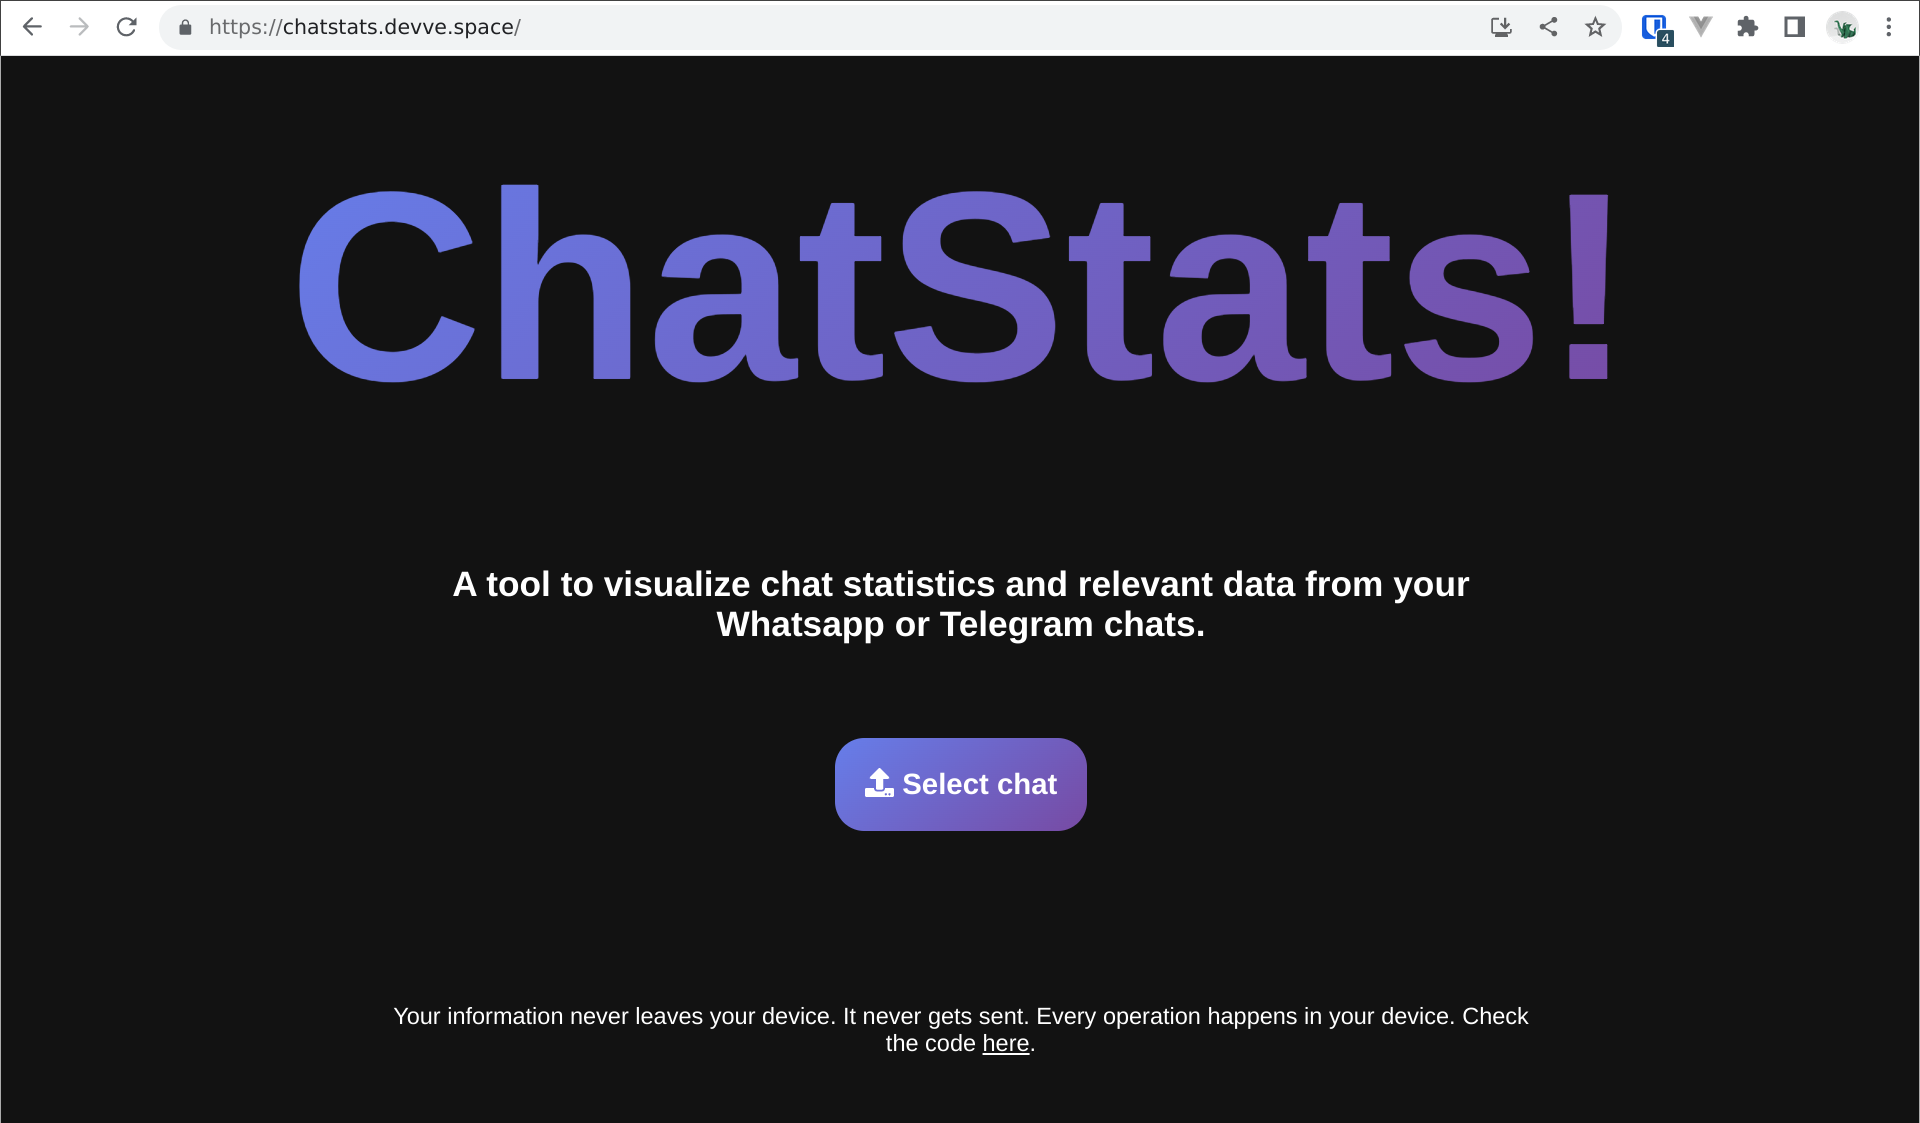
\includegraphics[width=0.95\textwidth]{img/study_case/step1.png}
	\caption{Página principal de la aplicación}
	\label{fig:chap5:step_1}
\end{figure}

En esta pantalla se describe la aplicación, así como una pequeña nota sobre la privacidad del servicio y un enlace al código fuente del mismo.


\subsection{Paso 2. Selección del archivo de datos conversacionales}

El usuario pulsa el botón para seleccionar un chat, lo que le abre el explorador de archivos de su sistema para seleccionar el fichero a utilizar.

\begin{figure}[H]
	\centering
	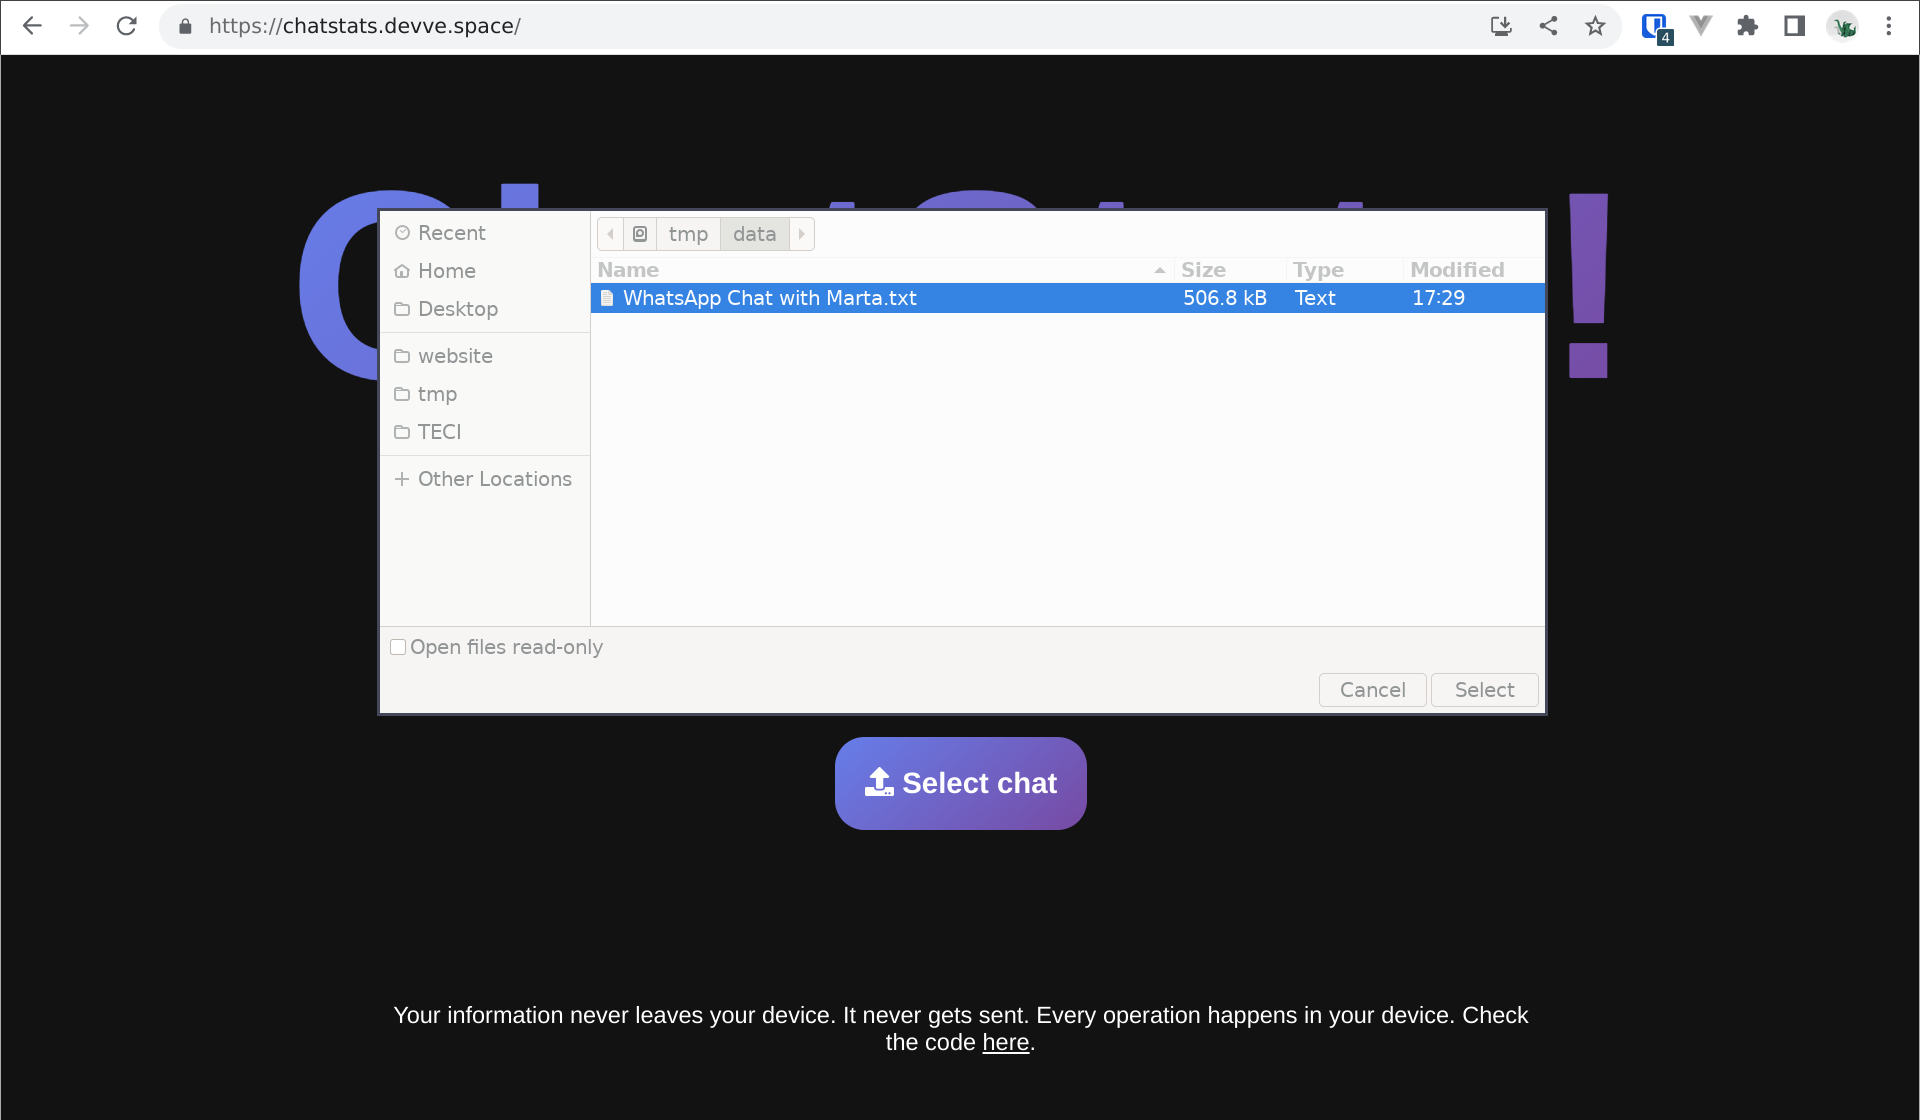
\includegraphics[width=0.95\textwidth]{img/study_case/step2.png}
	\caption{Selección del fichero de datos conversacionales}
	\label{fig:chap5:step_2}
\end{figure}


\subsection{Paso 3. Confirmación del archivo seleccionado}

Se muestra al usuario el nombre del archivo que ha seleccionado y se añade un botón para comenzar el análisis de los datos.

Asimismo, el botón para seleccionar un fichero sigue habilitado, permitiendo al usuario cambiar el archivo que ha seleccionado.

\begin{figure}[H]
	\centering
	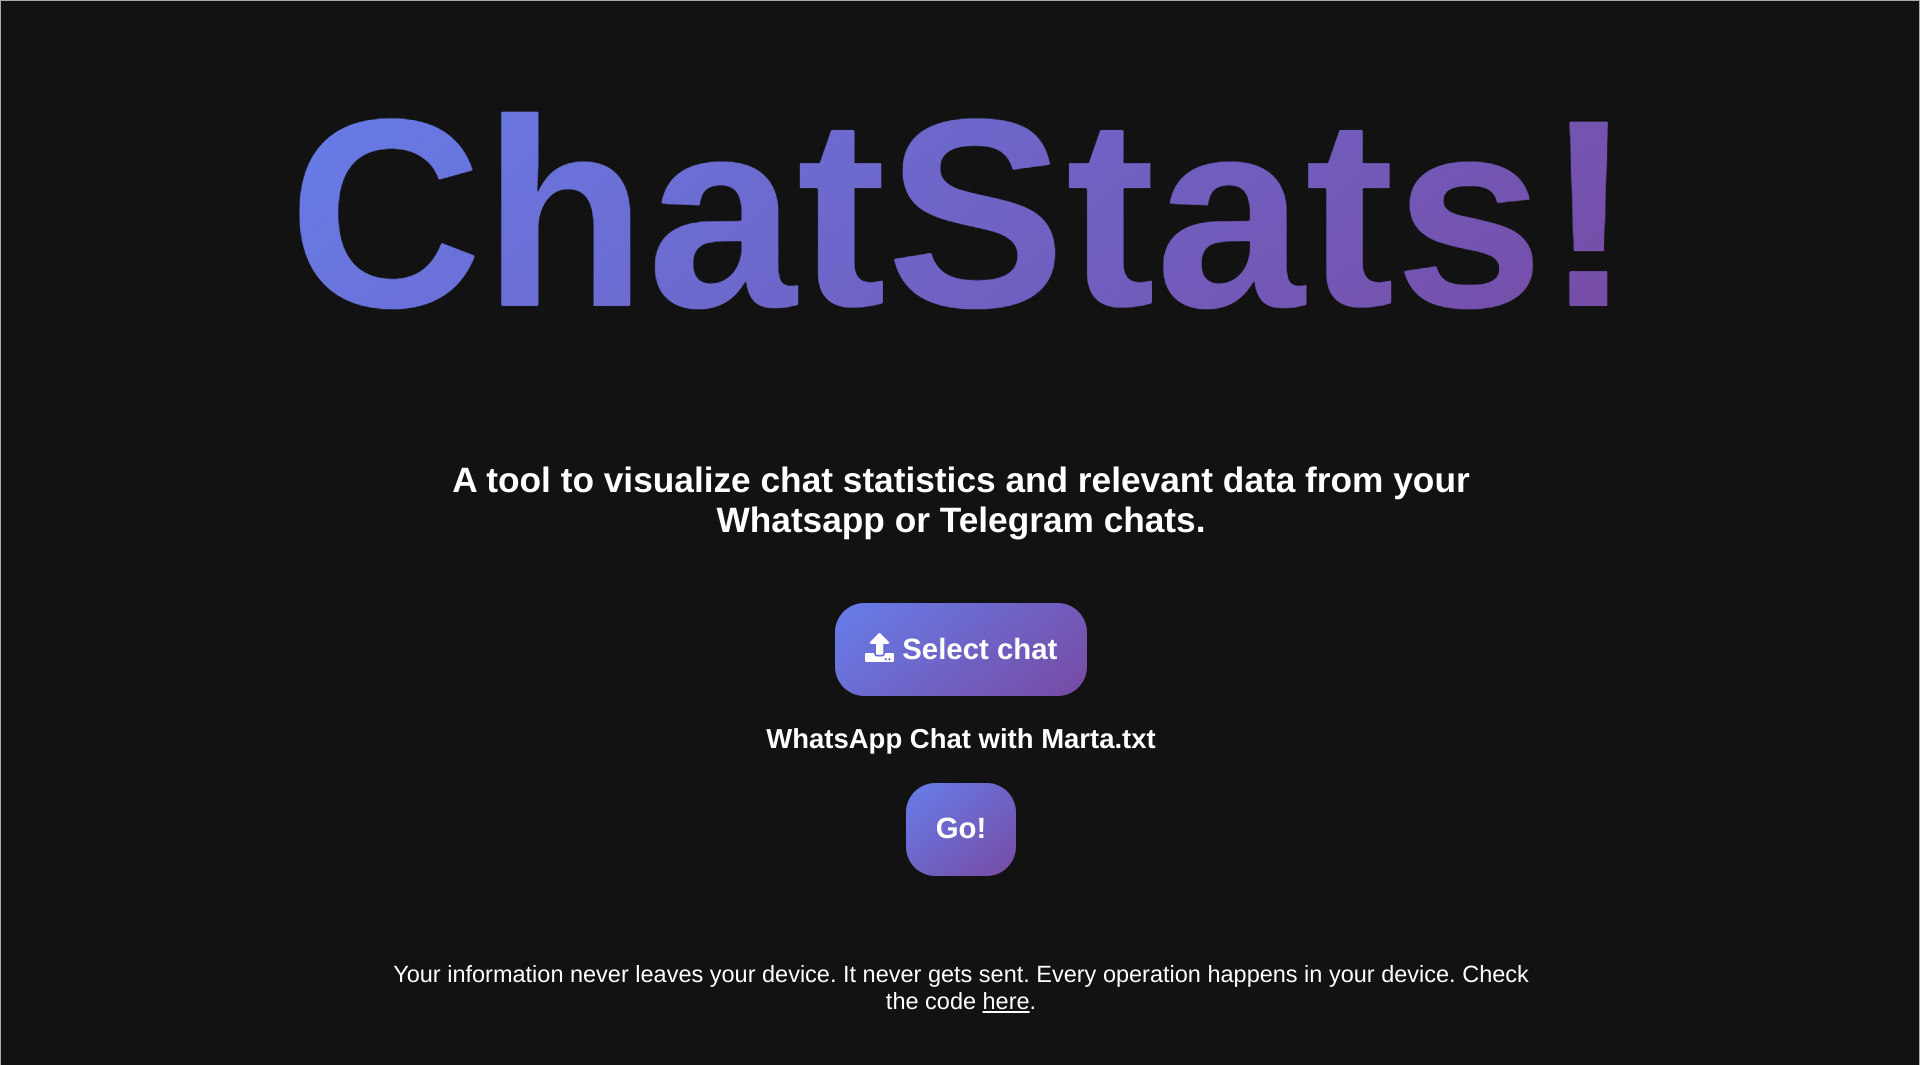
\includegraphics[width=0.95\textwidth]{img/study_case/step3.png}
	\caption{Confirmación de la selección}
	\label{fig:chap5:step_3}
\end{figure}


\subsection{Paso 4. Cálculo de las estadísticas}

Durante esta pantalla, el cliente está ejecutando todos los flujos descritos en el \autoref{chap:architecture}. Se muestra una animación de carga para hacer saber al usuario que el cliente está realizando operaciones.

\begin{figure}[H]
	\centering
	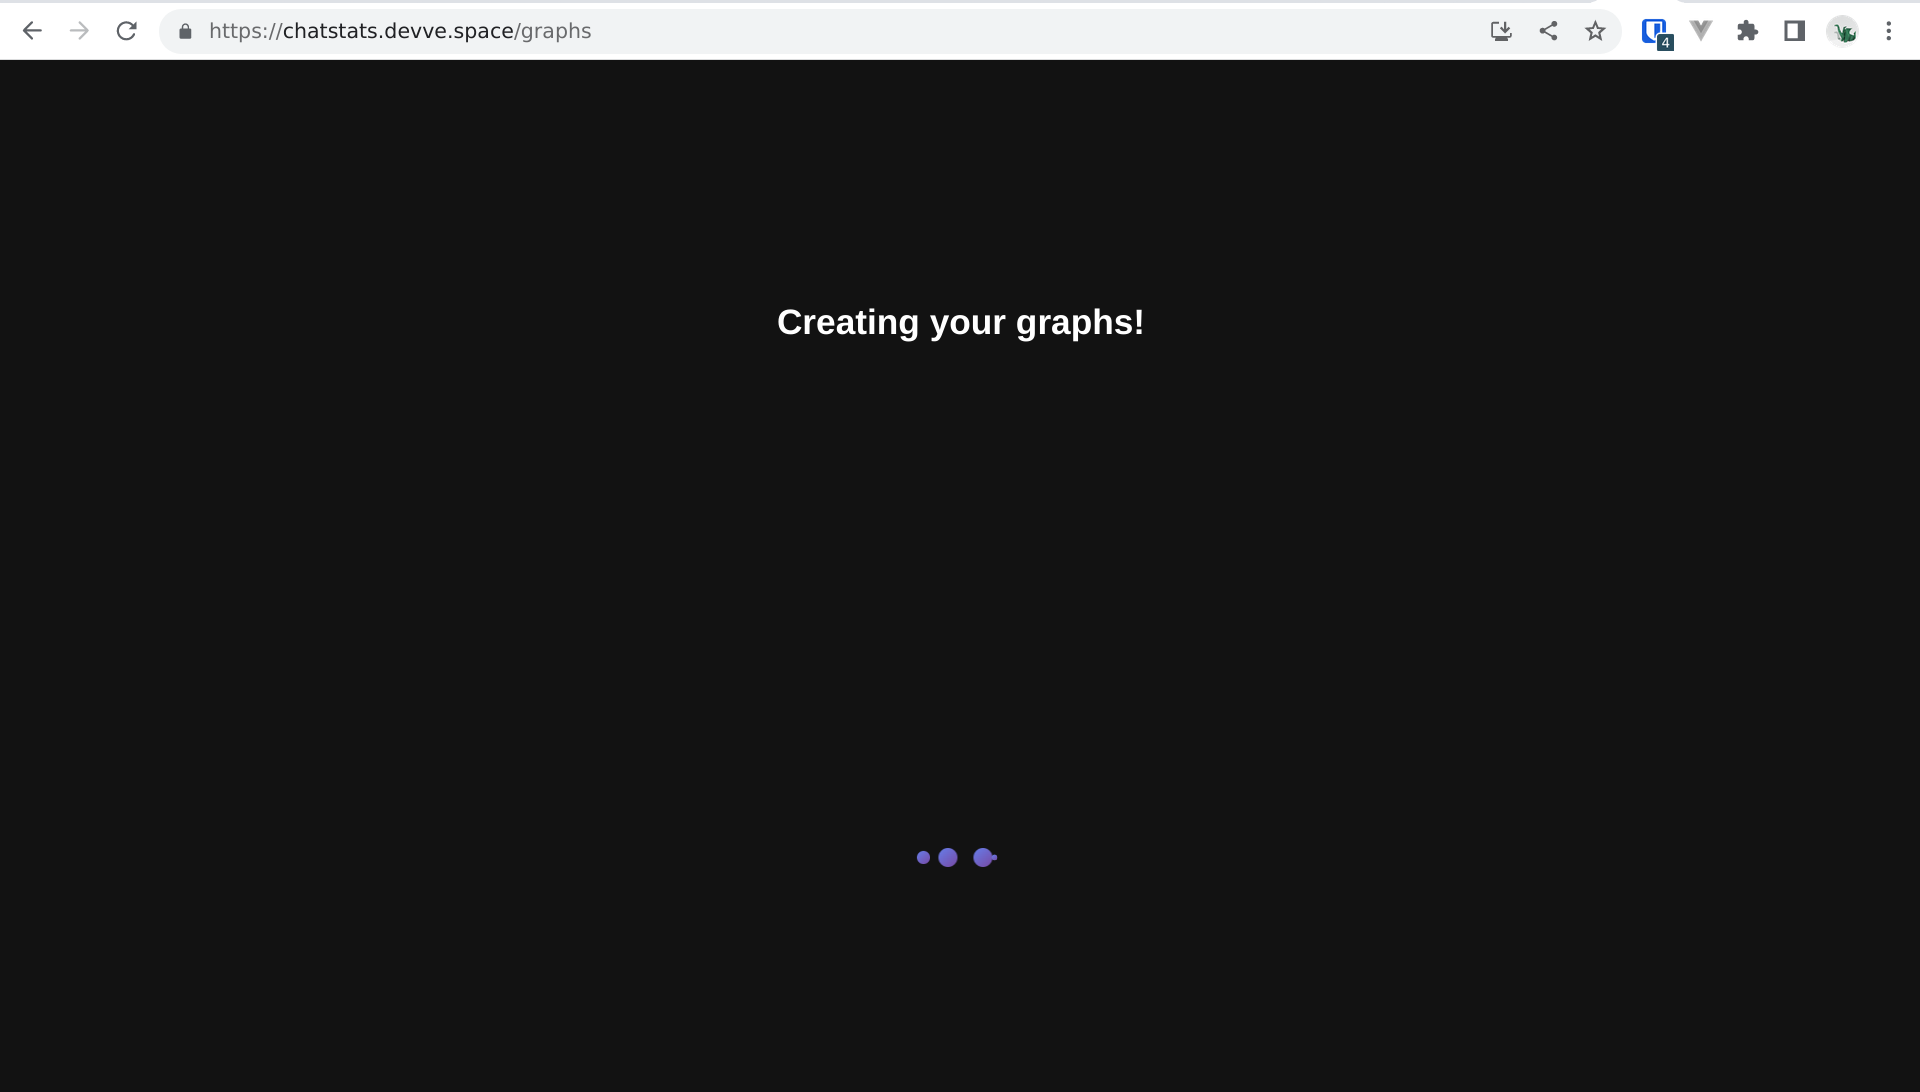
\includegraphics[width=0.95\textwidth]{img/study_case/step4.png}
	\caption{Cálculo de las estadísticas}
	\label{fig:chap5:step_4}
\end{figure}


\subsection{Paso 5. Visualización de estadísticas y gráficos}

En esta página se muestran numerosos gráficos, por los que el usuario puede desplazarse mediante la navegación vertical.

Los primeros gráficos tratan del recuento de mensajes y caracteres totales, así como la media de los mismos por cada mensaje.

\begin{figure}[H]
	\centering
	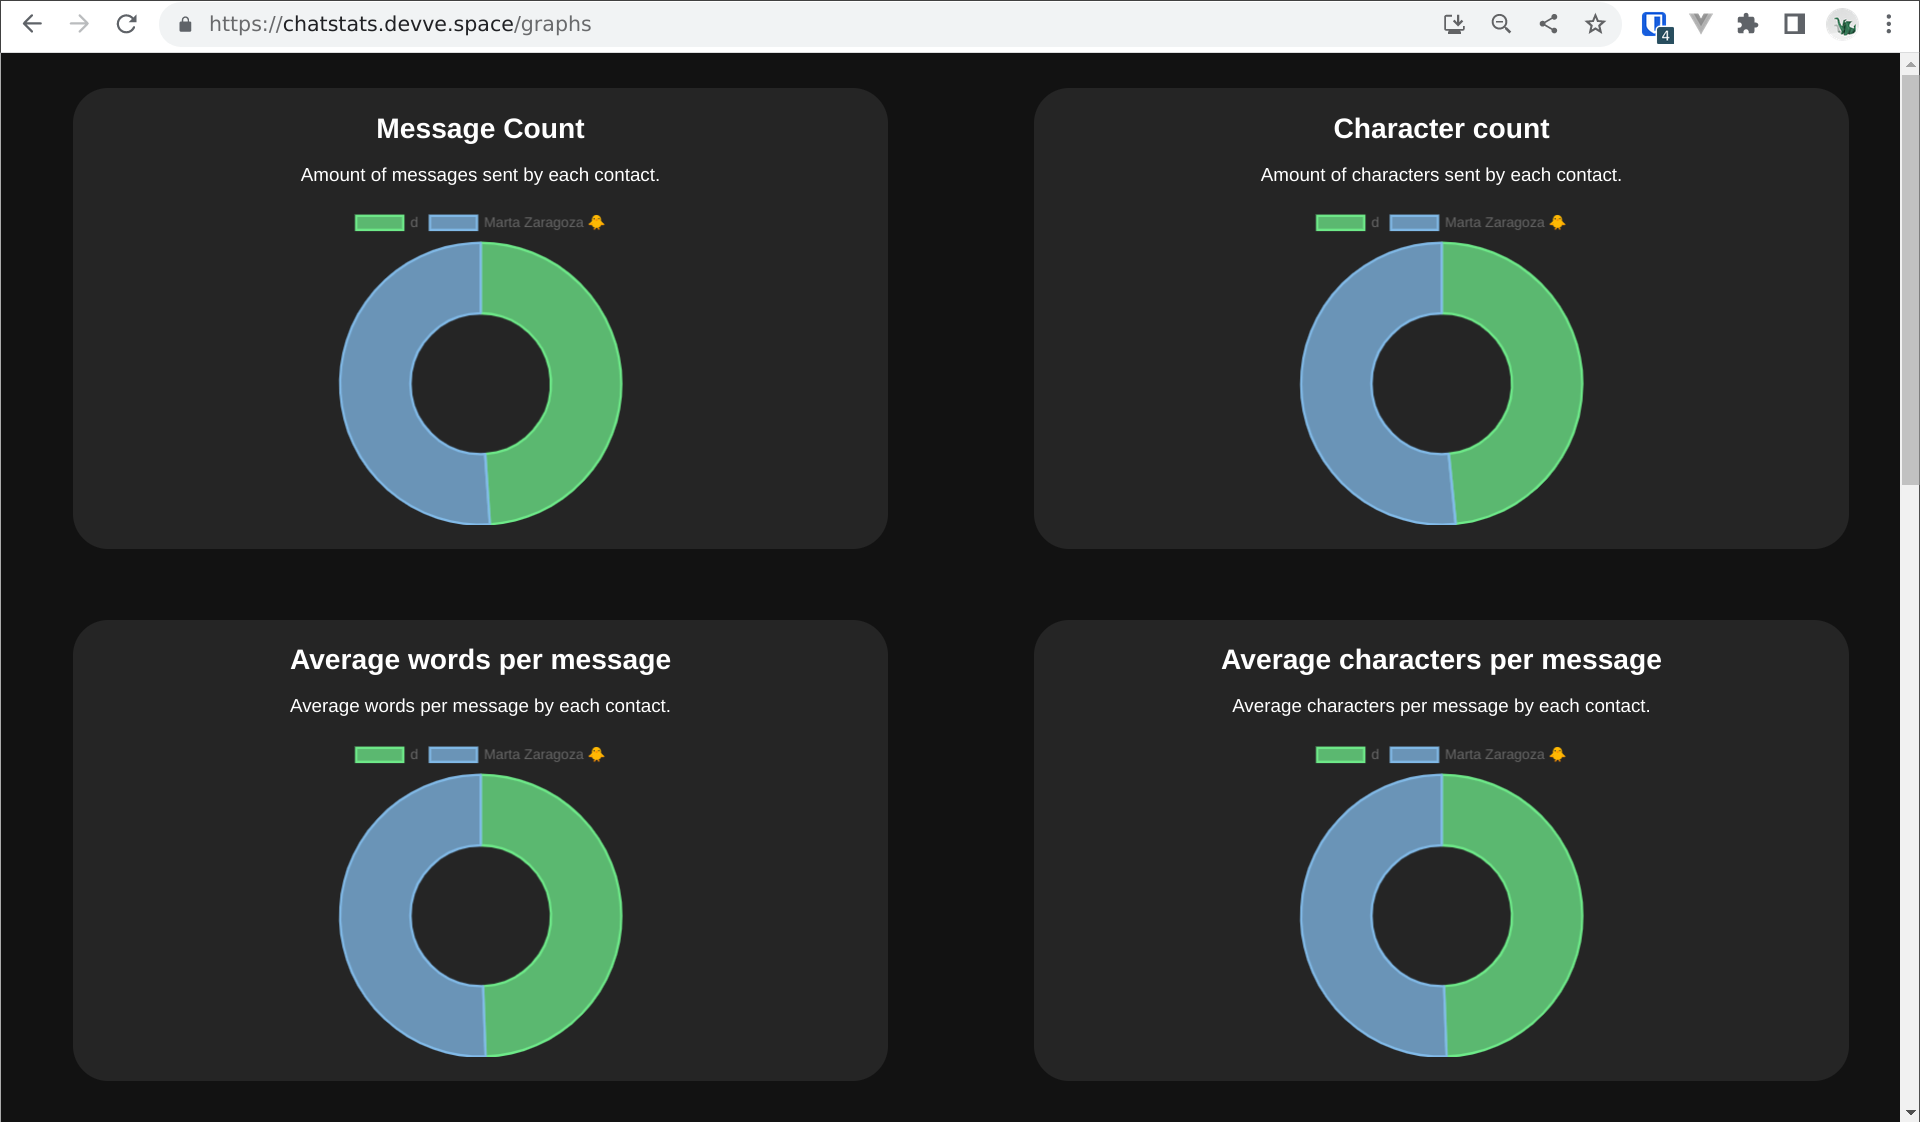
\includegraphics[width=0.95\textwidth]{img/study_case/step5_1.png}
	\caption{Cálculo de las estadísticas}
	\label{fig:chap5:step_5_1}
\end{figure}

Continuando más abajo, se muestra la distribución de los mensajes por contacto para cada mes, así como la distribución de los mensajes en media a lo largo de la semana. Finalmente, también se muestra la distribución de los mensajes en las horas en las que se envían.

\begin{figure}[H]
	\centering
	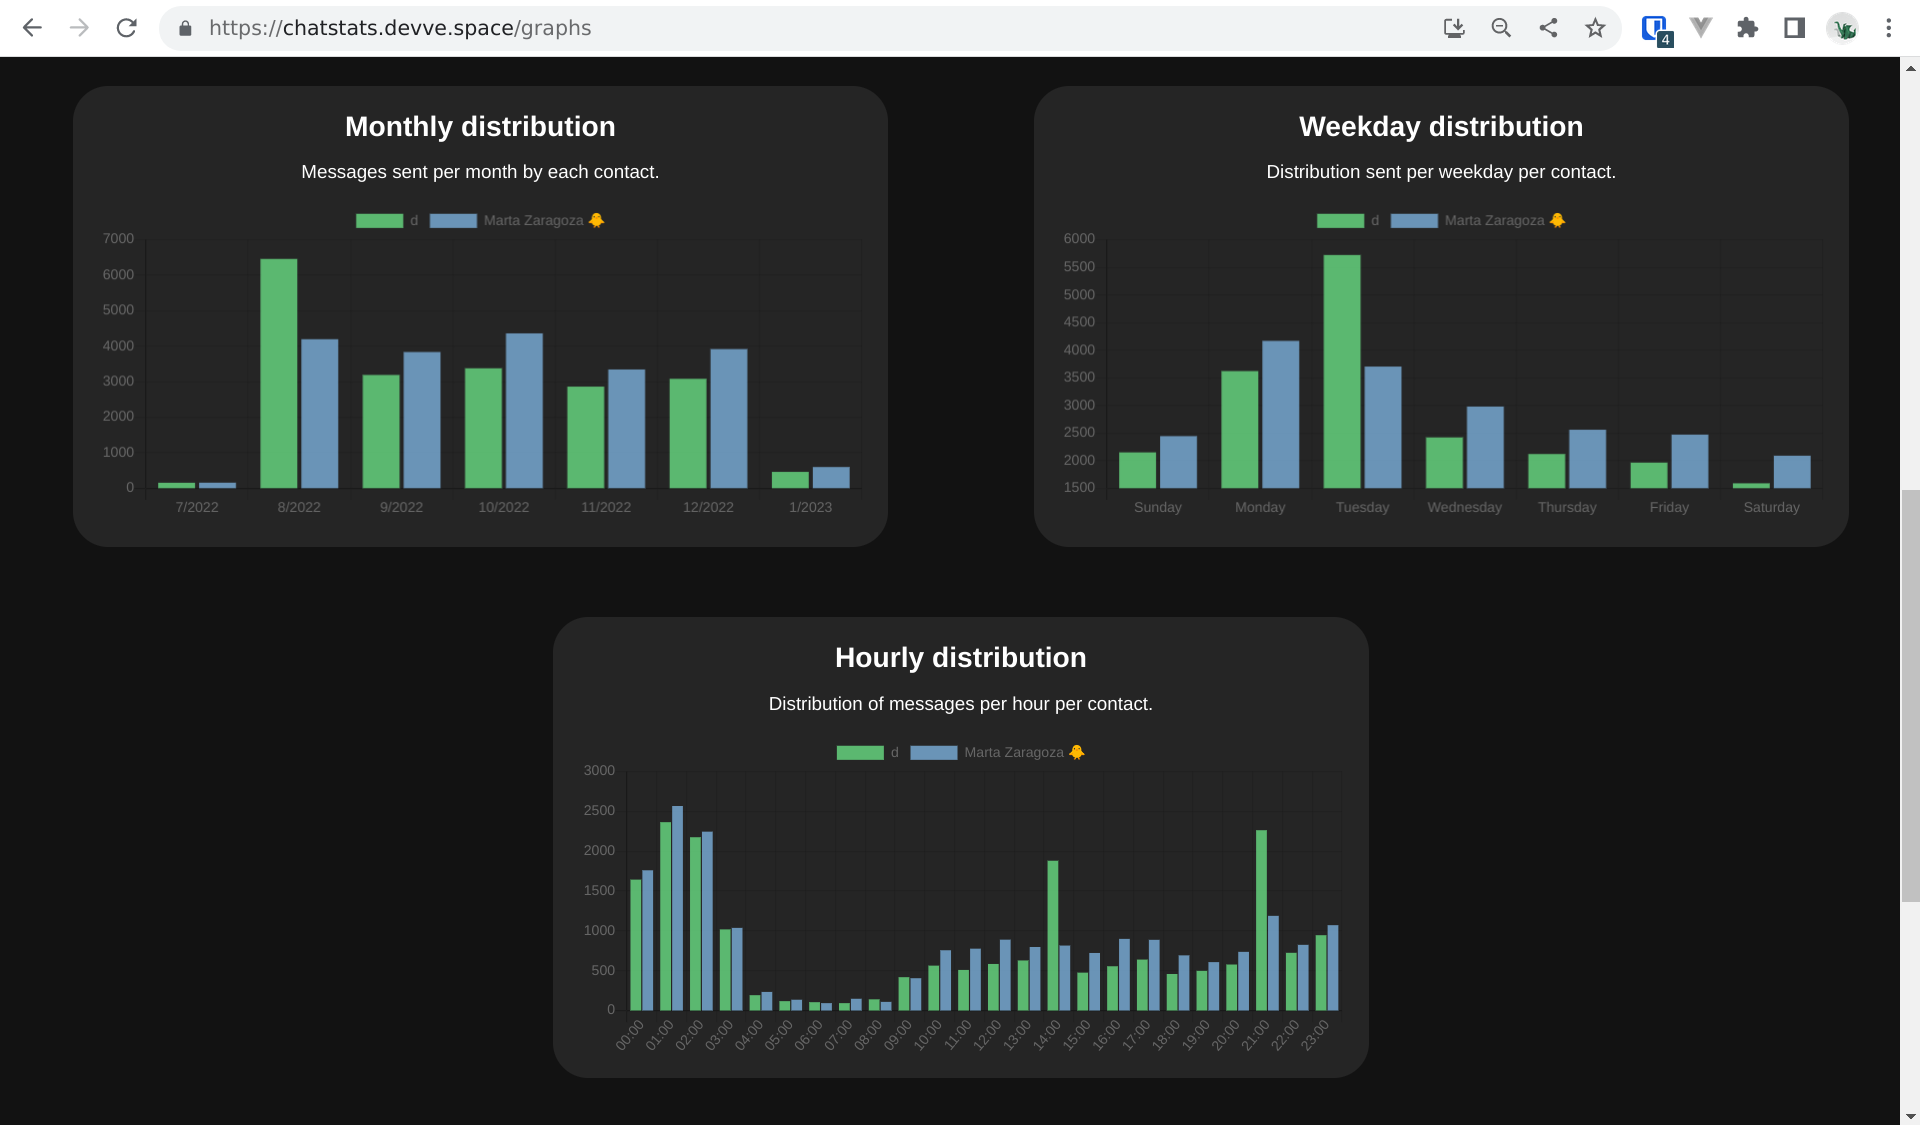
\includegraphics[width=0.95\textwidth]{img/study_case/step5_2.png}
	\caption{Cálculo de las estadísticas}
	\label{fig:chap5:step_5_2}
\end{figure}

Al final de la página se introducen dos gráficos más.

La nube de palabras muestra las palabras más utilizadas en el chat, teniendo mayor tamaño las palabras más utilizadas.

La nube de emoticonos o, \textit{emojis}, realiza la misma acción con los emoticonos.


\begin{figure}[H]
	\centering
	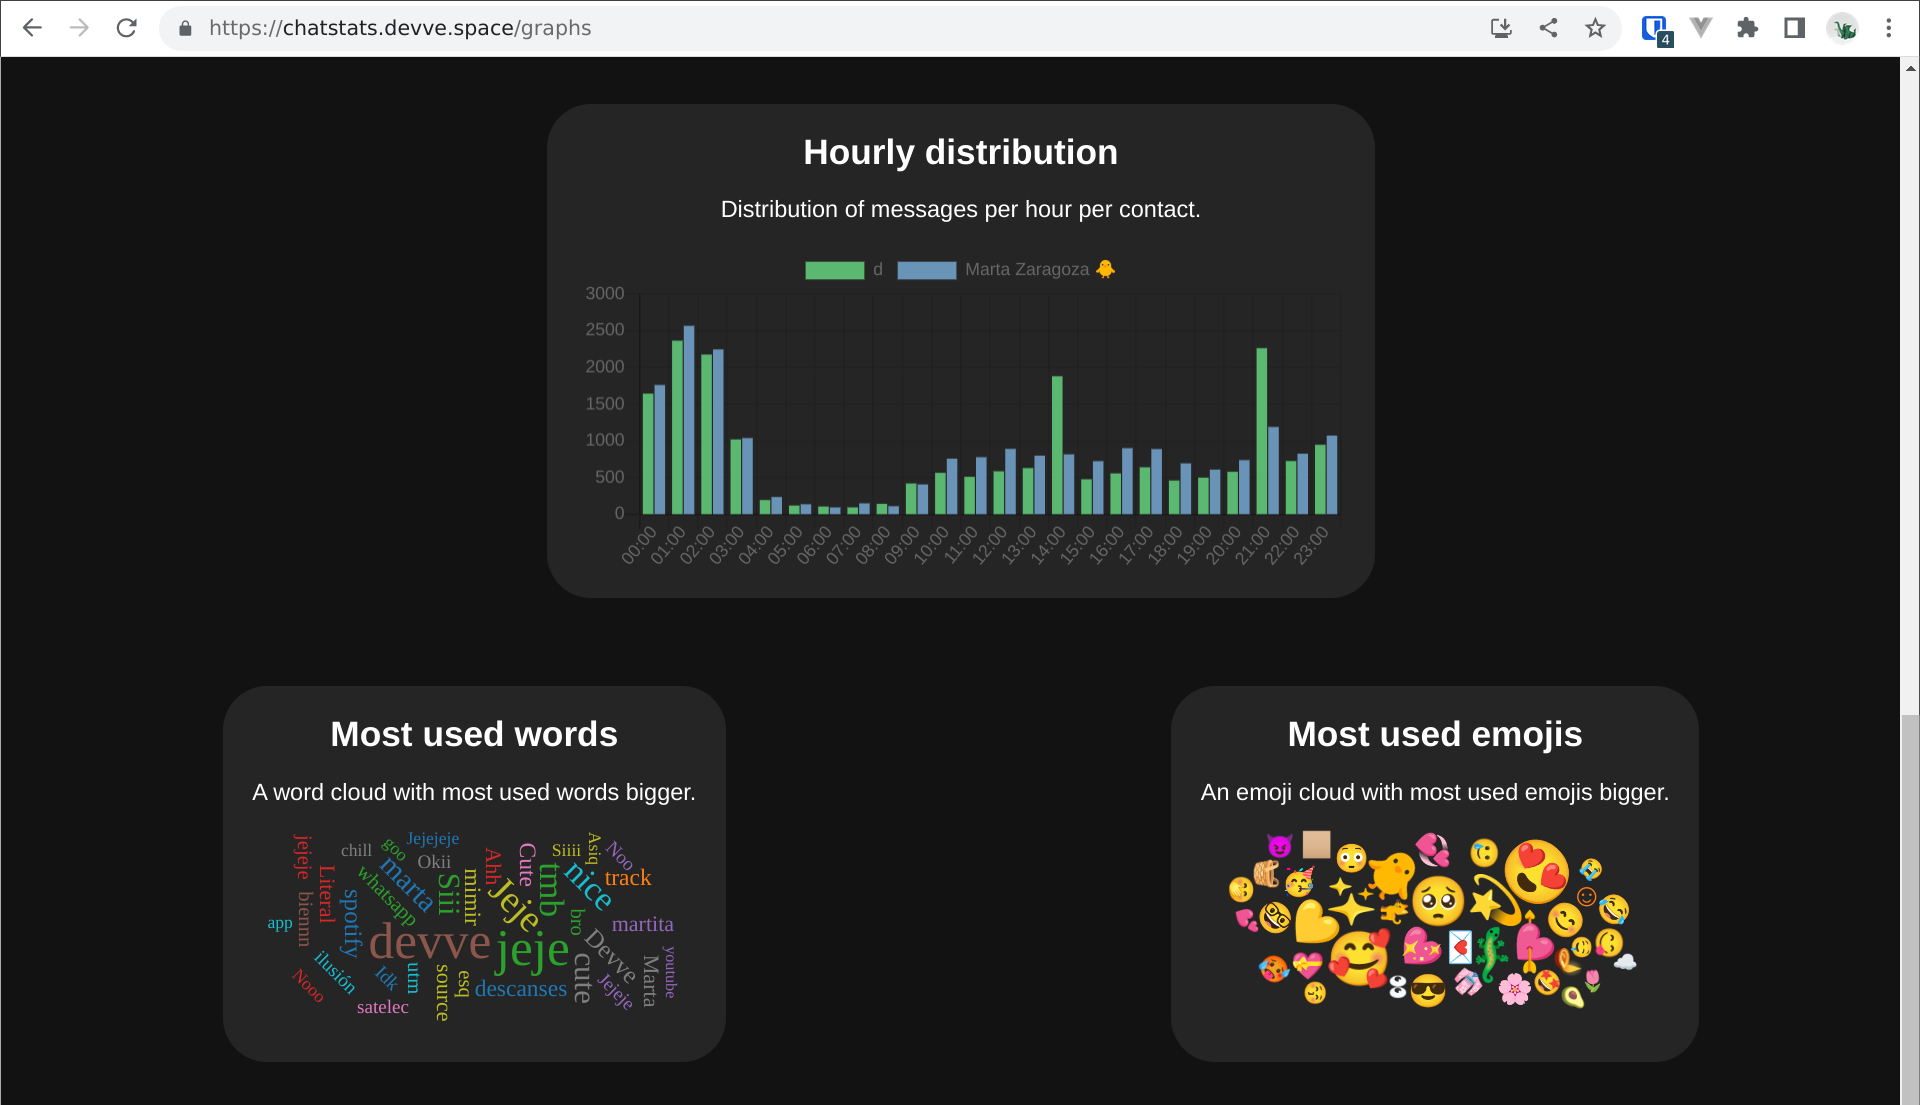
\includegraphics[width=0.95\textwidth]{img/study_case/step5_3.png}
	\caption{Cálculo de las estadísticas}
	\label{fig:chap5:step_5_3}
\end{figure}